\renewcommand\thetable{\arabic{chapter}-\arabic{table}}
%\renewcommand\thefigure{\arabic{chapter}-\arabic{figure}}
\renewcommand{\theequation}{\arabic{chapter}-\arabic{equation}}
\chapter{校舍耐震資料庫}

學校是人才培育的場所,也是緊急災難時,居民避難的主要地方,但台灣地區學校建築在每次大地震來時之損壞卻非常嚴重,尤其是老舊校舍,因興建年代久遠,其設計時所依據規範較為老舊,耐震能力可能遠低於現今結構耐震安全上之要求,故教育部已委託國家地震工程研究中心進行全國學校校舍之耐震能力評估與補強研究,此研究計畫著眼於校舍建築耐震能力評估補強機制及施行細節的建立,以對全國學校校舍耐震能力作一全面性普查,以篩選出耐震有疑慮之校舍,並儘速透過補強或拆除新建的手段來提昇校舍的耐震能力。而此計畫進行期間所產生之資料,均收集到此一校舍耐震資料庫中。

\section{收集範圍}

此一校舍耐震資料庫中收集有台灣各級學校,不同詳細程度的耐震能力相關的調查資料,此一資料庫乃是由國家地震工程研究中心(NCREE)在執行教育部委託之「全國各級學校舍耐震能力補強計畫」時所建。而除了耐震能力相關的結構評估資料,本資料庫還收集了評估階段之後的,包括補強設計、補強工程發包與結案的相關資料。

結構耐震能力評估的方法可分為兩類,第一類為初步評估(preliminary evaluation),其通常的方法是基於結構物之設計及現況填寫評估表,所填寫資料再依評估公式計算出結構物耐震能力之評分等級或指數,此類方法之評估速度快,但是結果可靠度較低,主要的目的是對大量結構物之耐震能力作排序與篩選,這類型評估方法所使用之評估表與評估公式通常是使用已經收集的其他結構物資訊,用數值統計的方法迴歸,或是根據基本的結構耐震能力供需比以及專業人士相關的經驗設計得到的,其所適用之結構物類型也有所限制,評估表並不能套用到各種類型的結構物上;另一類評估方法為詳細評估(detailed evaluation),此類方法為對結構物進行詳細的結構耐震分析,通常是使用結構分析程式以電腦數值模擬結構物遇到地震時的非現性行為,並根據模擬結果為依據,準確詳細的檢驗評估出結構物的耐震能力,這類方法的可靠度較高,但是花費相當昂貴,所需要的時間也比使用評估表要來的久很多。此二類耐震評估的方式通常相輔相成,結合成為標準的結構耐震能力評估程序,其即是先對所有需評估之結構物先以初步評估作耐震能力之評分與排序,以篩選出其中耐震能力有疑慮者,再對其以詳細評估的方式做詳細的檢驗。

由於中小學校舍數量龐大,若直接大量投入人力物力,可能造成大量之資源浪費,也無法快速的鎖定耐震能力不足之校舍建築,故針對有效達成此一校舍耐震評估標準需求以及基於上述標準耐震評估程序之精神,國家地震工程研究中心提出之解決程序為;經由學校總務人員之簡易調查及工程專業人員之初步評估,有效的將校舍結構之耐震能力排序,以縮小問題之規模,對於耐震堪慮之校舍,依嚴重程度,由工程專業人員,進行結構耐震之詳細評估,倘尚符合補強之經濟效益,即進一步作耐震補強之設計,若不符合補強之經濟效益,則將之列為拆除重建。在此過程中會產生的校舍資料最重要的為:初步評估、詳細評估、補強設計、補強工程等四組資料。

\subsection{初步評估}

由於本國之校舍建築有極大比例在校舍的結構形式、幾何尺寸等都有相似的結構,其平面配置多如圖\ref{fig:TSB},這類校舍為一字型的長形建築,教室一間一間排列,教室外有走廊,走廊可能有柱,且樓層數多不超過五樓,此一類型之校舍被稱為典型校舍,需要儲存的特徵值少,不用詳細記錄建物所有的樑柱牆等元件之相對位置,地震破壞時通常破護樓層都在一樓,而且是沿著長向破壞。在了解校舍常見的形式後,地震中心便以校舍結構物所能提供的耐震能力與需要的耐震能力相比的比值 $CDR$ 值為基礎,根據過往的實驗結果為依據,建立出校舍耐震能力的初步評估調查表。

\begin{figure}[hbtp]
  \begin{center}
    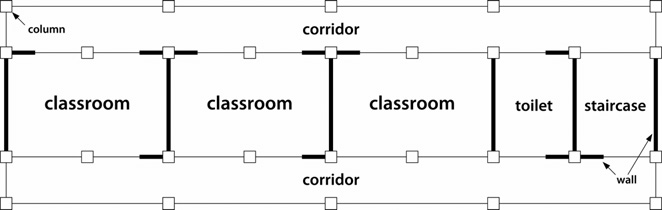
\includegraphics[width=1.0\textwidth]{figures/trad-school-buildings.png}
    \caption{典型校舍} 
    \label{fig:TSB}
  \end{center}
\end{figure}


\subsection{詳細評估}

ATC-40\cite{applied1996seismic}

耐震能力索引($CDR$)

\subsection{補強設計}

\subsection{補強工程}

